% !TEX root = 0main.tex
\section{Study Design}
\label{sec:study_design}

To understand the motivations behind the creation and maintenance of variant forks we conducted an online survey with maintainers of variant forks. In this section, we explain how we (i) designed the survey protocol; (ii) collected mainline--variant pairs and extracted the maintainers of the variant forks; and (iii) recruited the survey participants.

%we  and then . Next, we designed and developed a survey protocol that we used to recruit the participants.
 %The survey was run in April 2021 with the goal of understanding why developers create and maintain variant forks.

\subsection{Survey Protocol Design}
\label{sec:protocal}

%Since our aim was to learn from a large number of participants, we opted to use surveys that scales well as compared to interviews.
%\tm{I do not understand the sentence "we opted to use surveys scale well", something is incorrect in this sentence.}
%Relying on the knowledge gained from literature, especially the motivations presented in Section~\ref{sec:motivations},
%\cd{I would drop the first part of the section, as you already had a stronger motivation for the survey in the beginning}
We designed a 12-question survey that would last at most 15 minutes.
Since we aimed to learn from a large number of projects, we used an online survey as this data collection approach is known to scale well~\cite{Flick:2014}.
The survey can be found here\footnote{\url{10.5281/zenodo.5855808}}.
The questions were designed to cover our two main research questions.
%We designed the questions in such a way that the participants could choose the  reason from the provided options that best suited their motivations for forking.
8 of the 12 questions were close-ended and respondents could answer them either via multiple choice or Likert scales.
%Some of the possible answers motivations we.
%\sd{The paper refers to times to "our literature review". Either add a sentence or a paragraph explaining what this literature entailed. Or otherwise drop completely}
An optional free-text form was provided for 3 of the 8 close-ended questions to allow respondents to share additional thoughts and feedback.
The 4 remaining questions are open-ended.
All questions were carefully formulated so as not to bias respondents towards a specific answer. We validated them by subjecting them to the critical eye of 7 colleagues and by conducting trial runs of the survey with the same 7 participants.%\tm{Can you be more precise than say "a limited group of"? Just provide the number.}

%\ad{@John: I believe it would be nice to provide a link to the survey to that readers can see exactly what we asked. If you do so, please remember that SANER follows a double-blind review process, so the survey should be anonymized.}\jb{could someone help with this.}


\subsection{Identifying variant projects and participants}
\label{sec:forks_and_participants}

Given the scope of the survey, we target respondents involved in the creation and maintenance of variant projects.
Therefore, we first needed to identify such variants.
To this end, we relied on two data sources: \librariesio and \gh.

\librariesio contains metadata about projects distributed through various package registries. We collected the metadata for all projects of some of the largest package registries (\textsf{npm, Go, Maven, PyPI} and \textsf{Packagist}). We relied on this metadata to identify those projects that are variants of another one, following the variant identification method proposed by  Businge et al.~\cite{businge:emse:2021,businge:benevol:2020}. %The authors argue that, if a fork has distributed its package releases on a package registries, then one can be certain that it is a variant fork and very unlikely to be social fork.
We only considered variants that are actively maintained in parallel with their mainline counterparts. We extracted variants for which the mainline--variant pair was created before 2019-04-01 and updated at least once after 2020-04-01 (i.e., active projects).
%\tm{The choice of this start and end date is not motivated.}
This process yielded \textit{227 mainline–variant project pairs}.

We collected additional mainline-variant pairs from \gh directly.
To do so, we searched for mainline projects using the \gh search endpoint. We looked for \emph{popular} ($>50$ stars and forks), \emph{long-lived} (created before 2018) and \emph{active} (still updated in 2020) repositories.
We focused on software development repositories whose main language is among the top 17 of most popular languages used in \gh (e.g., \textsf{JavaScript, Java, Go, Python, Ruby, C}, etc).
For all the mainline projects we found, we tried to  identify and collect variant forks. This process is subject to a known threat to validity since previous studies revealed that the majority of forks on \gh are inactive~\cite{businge:2019Saner,Businge:2017} or are social forks~\cite{businge:2018icsme}.
To reduce this threat, we filtered forks based on  the following heuristics: $\geq 10$ stars, $\geq 10$ commits ahead of the mainline, $\geq 5$ closed pull requests, diverging \textsf{README} files.
%\cd{Here I would list all heuristics used rather than use examples and remain vague.}
We manually verified these remaining forks to ensure they corresponded to variants  of the corresponding mainline.
This process yielded \textit{264 additional mainline-variant project pairs},
leading to \textbf{a total of 491 collected mainline--variant pairs}.

% Furthermore, since we had to manually verify the final dataset as well as reduce the number of false positives, we came up with restrictive magic numbers to achieve our goal.
% We searched mainline repositories written in the 17 popular programming languages on \gh that include: \textsf{JavaScript}, \textsf{Java}, \textsf{Go}, \textsf{Python}, \textsf{Ruby}, \textsf{C}, having $>50$ forks and and also having a long development history (created before 2018-04-01 and updated after 2020-04-01).
% For each mainline, we extracted forks that were created before 2019-04-01 and updated after 2020-04-01, having $\geq 10$ stargazers, having $\geq 10$ commits ahead of the mainline (unique commits), having $\geq 5$ closed pull requests, and where the fork and mainline differ in the contents of the \textsf{readme.md} file for description.
% We manually verified that the mainline and fork indeed belonged to two different projects by reading and comparing the contents of their \textsf{readme.md}. Using this process, \textit{we obtained an additional 225 mainline–variant project pairs}.

%The mainline-variant project pairs we obtained so far correspond to \emph{attached forks}, in the sense that a direct traceability link exists between the mainline repository and the variant fork (i.e., the variant repository is \emph{officially} a \emph{fork of} the mainline repository on \gh).
%In contrast, \emph{detached forks} correspond to those repositories that were ``manually'' cloned from the mainline's one with no technically explicit traceability link.
%In the following, we will distinguish between two kind of variant projects, corresponding to \emph{attached forks} and \emph{detached forks}.
%\emph{Attached forks} correspond to those projects that are still \emph{attached} to the mainline in the sense that a direct traceability link exists between the mainline and fork (e.g., the \emph{fork of} attribute in \gh). On the other hand, \emph{detached forks} are those forks that were ``manually'' cloned and, consequently, whose repository does not maintain a link with the mainline.
%\ad{@John: Here we need to have some words to explain why you wanted to have \emph{detached forks} as well. It might be good to add an example of such a \emph{detached fork}.}

%To identify such detached forks, we relied again on \gh search endpoint. We searched for repositories that are not labelled as ``forks'' by \gh but that do contain ``\emph{fork of}'' in their description. We filtered out the resulting repositories the same way we did before with attached forks. We then manually inspected these repositories and manually identified the mainline projects they are variant of.
%\nd \textit{Identifying detached variant projects}. We used \gh search feature looking for repositories that are not referred as ``forks'' but that do contain ``fork of'' in their description and both the mainline and variant projects are actively maintained (i.e., were forked before \texttt{2019-04-01} and updated after \texttt{2020-04-01}; the mainline and variant have at least 100 commits after the fork date). We also manually verified that indeed the mainline and variant are indeed different projects being maintained in parallel by reading their \texttt{readme.md} pages. Using this process,
%This lead us with \textit{40 additional mainline–variant project pairs}.


\subsection{Participant Recruitment}

Based on this collection of mainline-variant pairs, we identified contributors that had integrated at least one pull request into the variant. % (i.e., contributors that are maintainers of the project).\tm{I removed the sentence between parenthesis, since it is hard to argue that you are a project maintainer if you only made a single PR!}
We retrieved their public-facing emails (if available) using the \gh API, while ensuring to respect the \gh Privacy Statement.\footnote{https://docs.github.com/en/github/site-policy/github-privacy-statement}
We individually contacted a total of 762 variant maintainers from the 491 variant projects, and received \textbf{a total of 105 responses (response rate 14\%), representing a total of 105 variant forks (21\%)}.
All participants were requires to read and accept an informed consent form before taking part in the survey.

%When distributing the survey protocol, we customized each of the \textit{email message content} using the respondents personal information. For example the email title was customized as follows\footnote{Academic Research on motivation of creating forks - \texttt{[fork\_name]}}. The body of the email message was also customized as follows\footnote{[\ldots] we have identified your \gh repository \texttt{[fork\_name]} as a variant fork of the mainline \texttt{[mainline\_name]}}.

\begin{figure}[ht]
\begin{center}
    \centering
    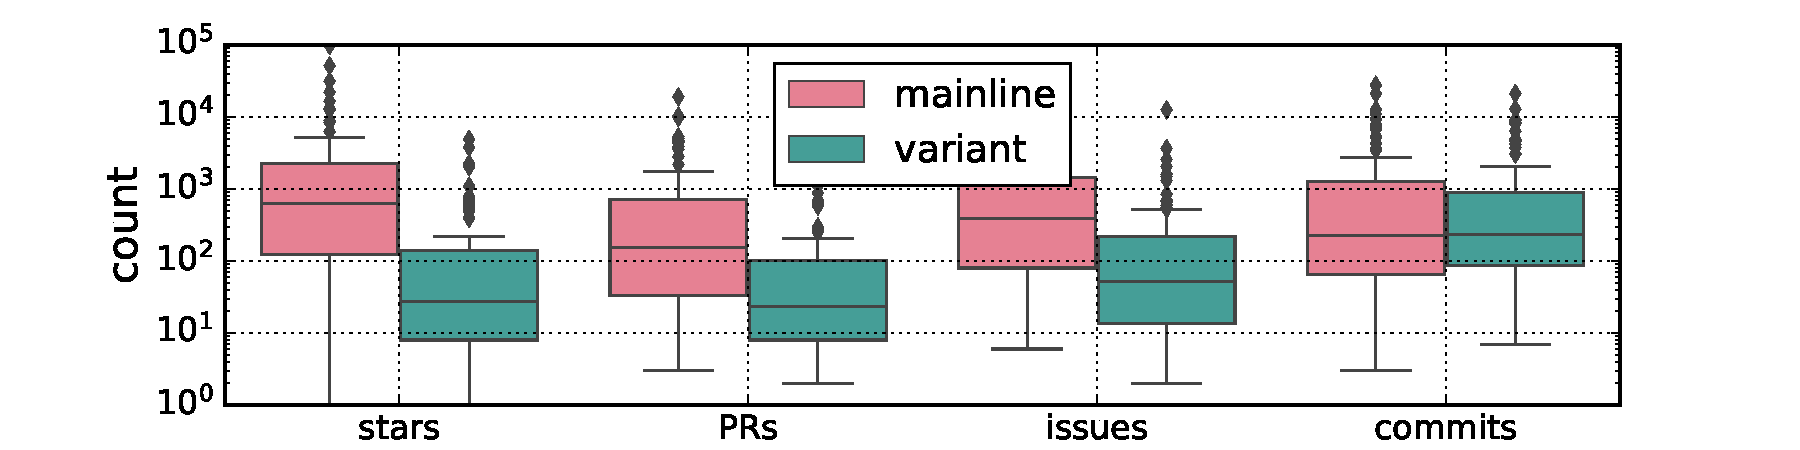
\includegraphics[width=\columnwidth]{pdfs/stats.pdf}
    \caption{Distribution of selected metrics. PRs, issues and commits are counted after the fork date for both mainline and variant.}
    \label{fig:stats}
\end{center}
\vspace{-.3cm}
\end{figure}

We wanted to compare the popularity of the 105 mainline--variant pairs since the fork date. To this end, we collected metrics of stars, pull requests, issues and commits from the projects. For the variant projects, all these metrics are calculated from the fork date. For the mainline projects, we calculate the metrics  of pull requests, issues and commits from the fork date. The number of stars in the mainline are calculated throughout the lifetime of the project.
The boxplots in Fig.~\ref{fig:stats} show the distributions of stars, pull requests, issues and commits for the selected mainline-variant pairs. %Only the 105 projects for which at least one maintainer took part in the survey were considered.
%We wanted to compare the mainline and variants since the
%\ad{@John: I could not rewrite the next paragraph because I do not really understand it (and its purpose). I guess we need at least one or two sentences to explain the goal of the figure, and what can be observed from it.}
%Apart from the stars where we consider all in the mainline, we count all (closed + open) PRs, issues, and commits (only main branch) after the fork date.
While it is not surprising that the counts for mainline metrics are always higher than those of the variants, it is interesting that most variants are also popular in stars, pull requests and issues counts. This gives us confidence that we are studying real variants as opposed to social forks.
%\ad{I propose to move Fig.~\ref{fig:stats} and the corresponding text to previous section.}


\subsection{Analysis}
\label{sec:card_sorting}

%\ad{@John: I'm not really used to card sorting, but I couldn't really understand the whole process you followed after having read the following paragraph. Please add some sentences to explain why card sorting is needed and which ``issue(s)'' it solves.}\tm{People that know card sorting know what it is used for. Others can look at the cited reference.}

We used open card sorting~\cite{zimmermann2016card}, on the 3 open-ended questions to identify common responses reported by the participants.
In the analysis, we grouped similar responses from the open-ended questions into themes.
We did not start with any pre-defined themes in mind, but instead derived the themes from the open-ended answers, iterating as many times as needed until reaching a saturation point. The first iteration of coding themes was performed by the first author of the paper, and any responses the first author was unsure of were decided by discussion with the second author. Once the first two authors agreed on the themes, a virtual meeting was set with all six authors to discuss the resulting themes and come to a negotiated agreement~\cite{Garrison:2006}. This  allowed us to remove duplicates and, in some cases, to generalize or specialize themes.
